\chapter{Methods}\label{chapter:method}
This chapter lays out the steps necessary for our experiment to evaluate explanations' fidelity towards spurious feature importance. 
After defining a causal model of the data and explanation generation process we construct the metrics we test both to yield a ground truth feature importance as well as the importance attributed in the explanation. We also describe how the experiment is conducted and through which analysis methods we compare the metrics.

\section{Causal Model}\label{section:causal_model}
One core aspect of our analysis is the combination of causal methods for data generation and ground-truth feature attribution. 
The main process includes a hyperparameter, such as the later discussed coupling ratio $\rho$, which one can intervene on, together with predictions and explanations generated for multiple trained instances of a model and its output. 
Within this greater structure, a subprocess constructs the image dataset with a structural causal model taking only $\rho$ as an input. While $\rho$ stays fixed for each model to be trained, it is a causal variable in the overarching structure. This way we create an array of causally generated datasets whose constitution only differs by this one variable. 

\subsection{Data Generating Causal Model}\label{section:data_gen_causal_model}
For the most exact comparison of attribution between a model and its explanation it is imperative to know the ground truth of the training data. A structural causal model (SCM) can define variables and the \textit{independent} mechanisms with which they interact precisely. We want to define an SCM that closely mirrors image generation processes as they happen in realistic scenarios. 
Explicitly using a generating SCM has previously been done to create or test new attribution methods \citep{Parafita2019, Wilming2023, Clark2023, Goyal2019, Reimers2019, Reimers2020}. A few other works evaluating XAI methods with a known ground truth have implicitly used structures akin to an SCM without defining it in causal language \citep{Kim2018, Yang2019, Arras2022}. 

The causal graph and its structural assignments used for our experiment are defined as follows: 
\begin{equation}
\label{eq:scm}
\begin{aligned}[c]
G&:=\eta^g \notag \\ 
N_w&:=\eta^w  \notag \\ 
N_s&:=\eta^s \notag \\ 
N_x&:=\eta^x  \notag \\ 
W&:=(\rho * G + (1-\rho)* N_w) \geq 0.5 \notag \\ 
S&:=(\rho * G + (1-\rho)* N_s) \geq 0.5 \notag \\ 
Z&:= \eta^z \\ 
\mathcal{X}&:= W + f_{image}(S, Z) + N_{x} \\
\end{aligned}
\begin{aligned}[c]
& \mathrm{with} \  \eta^g \sim \mathcal{N}(0.5,0.02) && \notag \\ 
& \mathrm{with} \  \eta^w \sim \mathcal{N}(0.5,0.1) && \notag \\ 
& \mathrm{with} \  \eta^s \sim \mathcal{N}(0.5,0.1) && \notag \\ 
& \mathrm{with} \  \eta^x \sim \mathcal{N}(0,0.05) && \notag \\ 
\\
\\
& \mathrm{with} \  \eta^z \sim \mathcal{U}(0,245760) && \notag \\ 
\\
\end{aligned}
\end{equation}

These assignments are visualized in the causal graph in \cref{fig:generating_scm}.
Variables of interest are the spurious (watermark) feature $W$ and the target (shape) feature $S$ as well as their combination, the image dataset $\mathcal{X}$. $N$ represent noise or unobserved variables, $G$ the generator confounding $S$ and $W$, and $Z$ a multivariate variable describing all other factors of the dataset. 

\begin{figure}[t!]
    \centering
    \includegraphics[width=0.9\textwidth]{pics/generating_scm.png}
    \caption[Data Generating SCM]{Data Generating Structural causal model.
        $\rho$ is not visible in the SCM. It determines the signal-to-noise ratio between the confounding $G$ and the noise variables $N_w$ and $N_s$ in the structural assignments. The noise terms of $Z$ and $G$ are not shown explicitly.}
    \label{fig:generating_scm}
\end{figure}

The SCM, as seen in \cref{fig:generating_scm} and \cref{eq:scm}, serves as a ground truth for our experiment. It is mostly an additive model using Gaussian distributions for the noise terms, except for $Z$ which uniformly at random selects other image generating factors like rotation, scale and position of a shape. Also, the function $f_{image}$ generating the images out of the latent factors and the shape is not further specified.

The meta-variable $\rho$ adjusts how much information is shared between the true class information (shape), which we name \textit{core feature} following \cite{Singla2022} and the watermark or \textit{spurious feature} through a shared common ancestor named \textit{generator} $G$. For each model, coupling ratio $\rho$ is fixed to later enable a comparison between models trained with different coupling ratios. 
A second parameter which we keep fixed for all experiments, determines how frequent the spurious feature is in the data. We set this parameter which can be seen as the \textit{prevalence} to one half, so that just as many images have a watermark as not. Notably, when $\rho$ is one this means that all ellipses will have the watermark and no rectangle will and when $\rho$ is zero there is no correlation of watermark and shape. 

It is important to note that this particular SCM is just one of many possible ways to model how spurious features might interact with core features. It attempts to follow the logic of how images are generated or selected in real datasets. Here, it particularly looks at pathways for the generation of Clever-Hans or watermark features, often present in image datasets \citep{Lapuschkin2019}. As visible in \cref{fig:equivalent_scm} different causal models can produce an equivalent distribution of the two latent factors in question (watermark and shape). One can think of more variations of SCMs which are able to produce the same correlation, so the choice of using the confounder version as in \cref{fig:generating_scm} is mainly due to its ease of implementation. It also lends itself best to the Clever-Hans task, because in this SCM there is no real causal effect between the core and spurious feature. It would therefore be ideal for the a neural network to ignore the spurious feature completely. Without assumptions about the generating mechanism though, the confounder case is not identifiable, or in other words, distinguishable from $W \rightarrow G \rightarrow S$ and $S \rightarrow G \rightarrow W$ because it is Markov equivalent to those scenarios. 
Although the presented collider case (\cref{fig:equivalent_scm}\textbf{a}) is theoretically distinguishable from the confounder case (\textbf{b}), one can not hope that a network which only has access to the intervened on (selected) data will recover this. Neither can we hence expect the explanation to make such a distinction.

The idea of investigating the effect of a coupling ratio $\rho$ was inspired by \citet{Clark2023}, who also used a \textit{signal-to-noise} ratio in their generating model. Instead of a confounding model their learned data instances are colliders of the label and a suppressor variable similar to \cref{fig:equivalent_scm} \textbf{a}. In their experiments the expected explanation importance of a suppressor feature ought to be zero, as long as the collider is not intervened on, but also when the suppressor and core feature are coupled through smoothing of the image. We contest this assumption, as it is not clear whether a neural network does not implicitly condition on this collider (which is the image set), therefore introducing correlation between the parent components through a different kind of selection bias. We disagree with their statement that a good explanation method ought to not attribute any importance to such suppressor variables. This is, as  \citet{Nauta2023} put it, a case of conflating external \textit{coherence}, i.e., ``agreement with human rationales'' \citep{Atanasova2020} with \textit{correctness} towards the model. As we are not aware of any explicit way in which deep neural networks differentiate between a suppressor or confounder variable, it is unwarranted to expect an explanation to explain something the model does not even conceptualize. 

The direction of causal links for image classification is, as can be seen from this example, highly debatable and shall not be the focus of this work. Whether the selection of the AI researcher reducing costs with free images resulted in classes being polluted with watermarks (\cref{fig:equivalent_scm}\textbf{a}), or whether a scientist marked x-rays with their diagnosis (\cref{fig:equivalent_scm}\textbf{b}) seems to not be distinguishable for ML models. 
Instead, we only want to find to what degree a neural network learns and attribution method explains the distribution generated by a particular SCM.



\begin{figure}[t!]
    \centering
    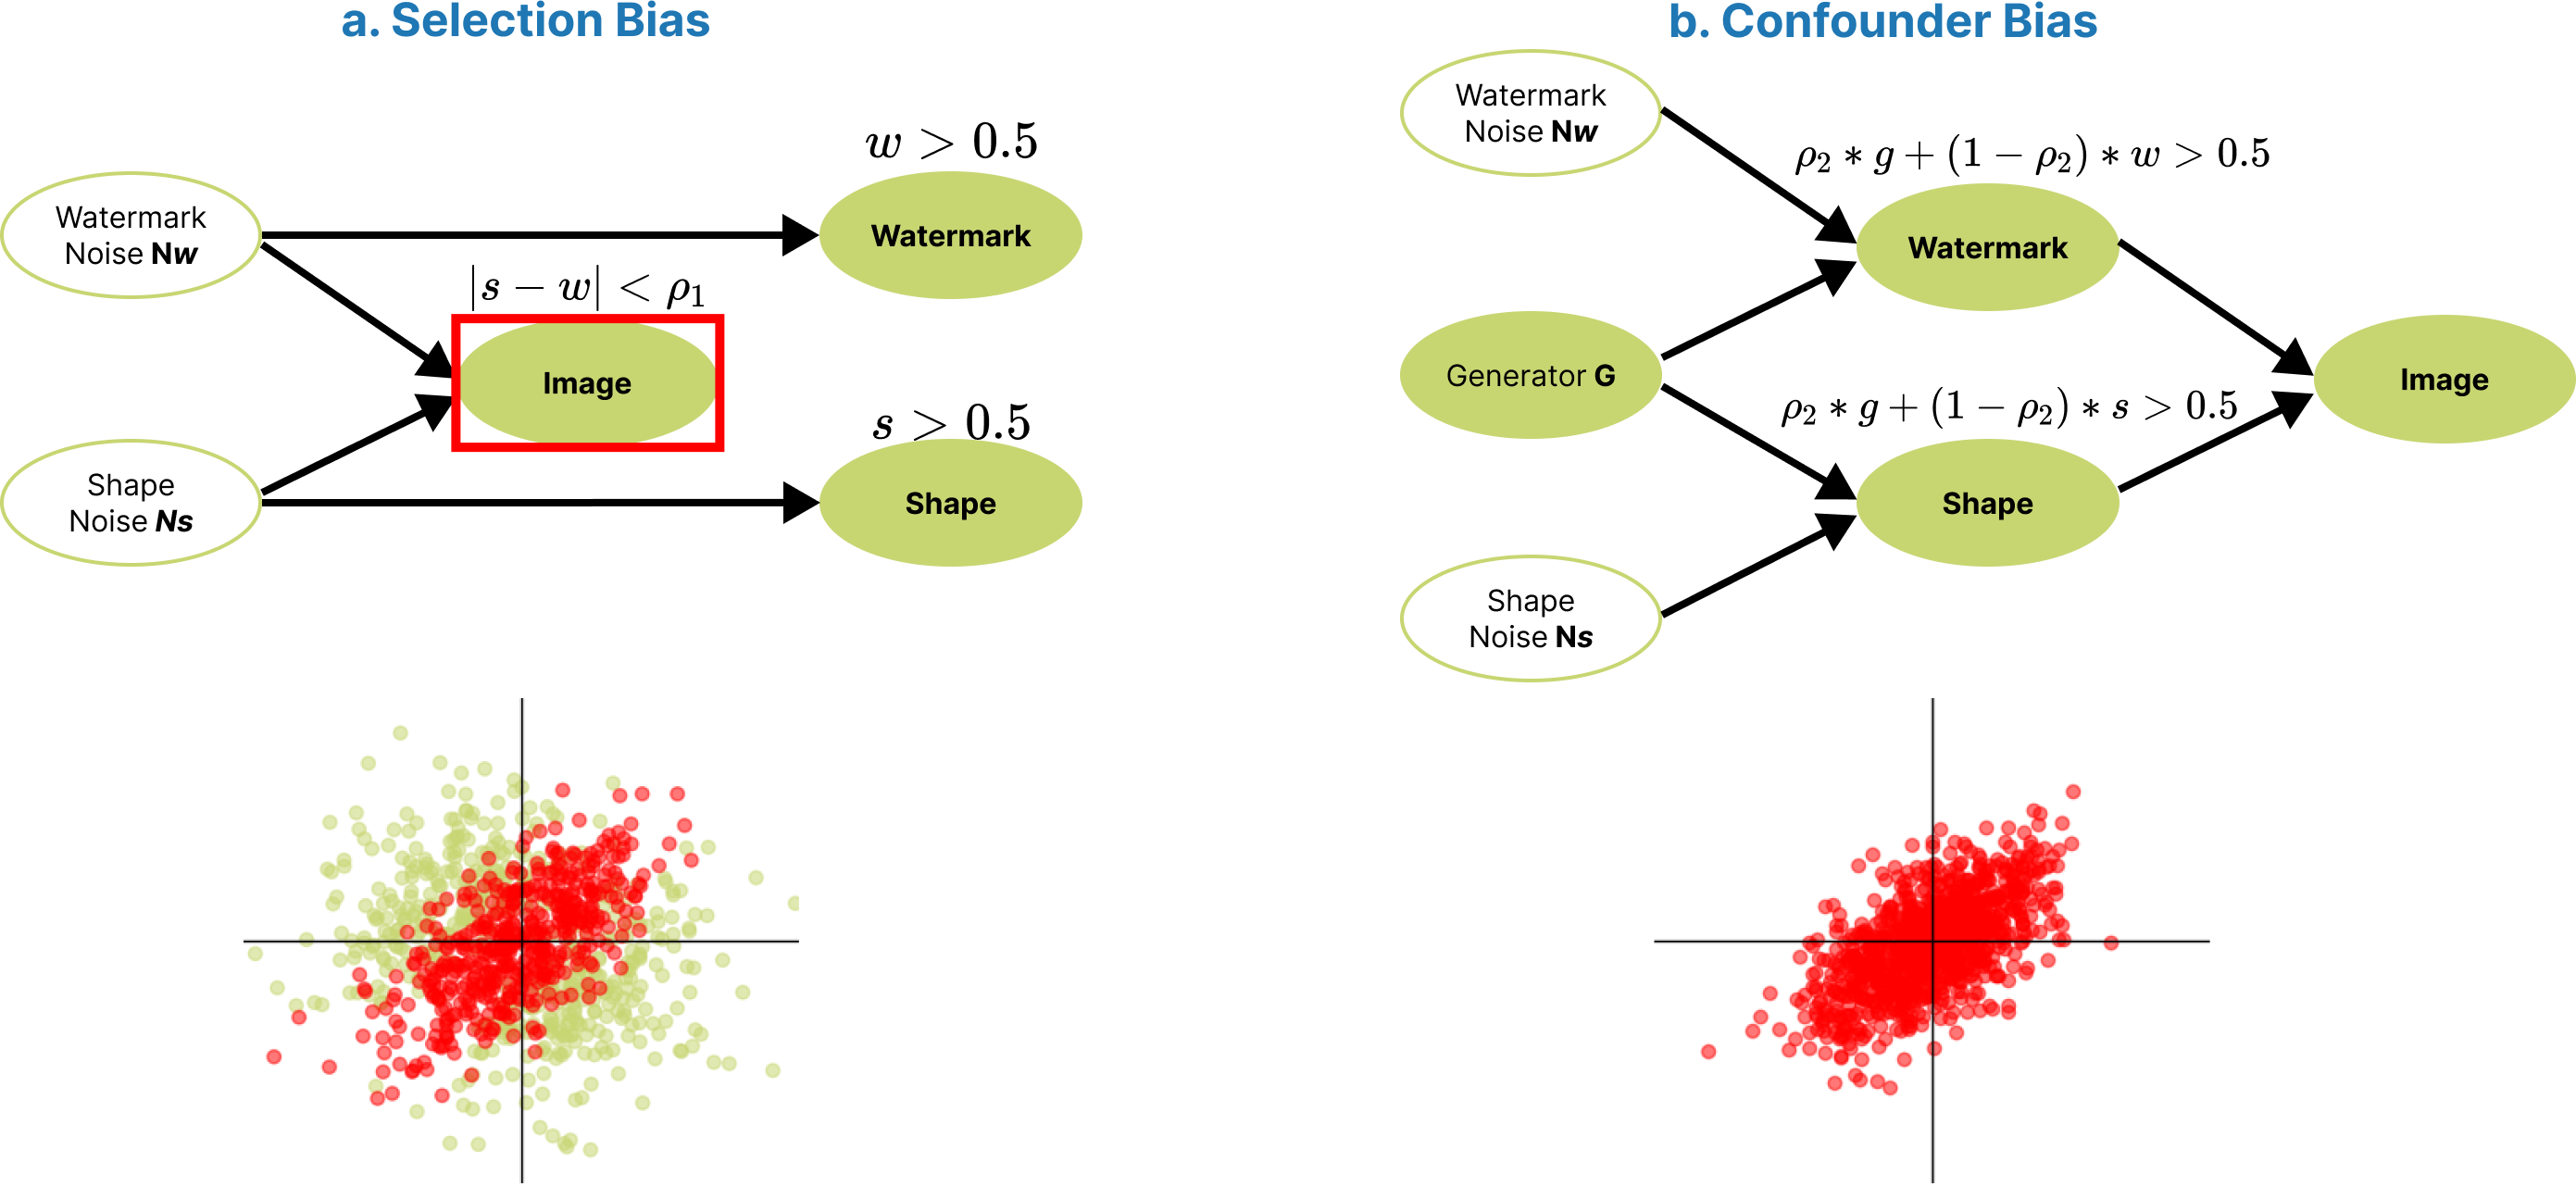
\includegraphics[width=0.8\textwidth]{pics/equivalent_scm.png}
    \caption[Selection vs. Confounder Bias]{SCMs typically found in image datasets.
    \textbf{a.} selection bias \textit{(researcher chooses images from free online collection with watermarks)}
    \textbf{b.} confounder bias \textit{(e.g. scientist marks positive x-ray scans with sign)}}
    \label{fig:equivalent_scm}
\end{figure}

\subsection{Explanation Generating Model}
The data generation causal model is part of the model which generates predictions and explanations.
This model is defined in a similar way to the \textit{explanation generating process (EGP)} by \citet{Karimi2023}.
Ratio $\rho$ is a meta-variable of our image generation process in a similar sense to how hyperparameters are defined for the training there. While \cref{fig:generating_scm} depicts the data generating causal model (DGCM) of the training dataset in more detail, \cref{fig:egp} shows how this is embedded into the mechanism of generating explanations. 

\begin{figure}[t!]
    \centering
    \tikzset{%
        neuron/.style={
            ellipse,
            draw,
            minimum height=8mm,
            },
        arrows={[scale=1.2]}
    }
%\begin{mdframed}[backgroundcolor=graybg]
    \begin{tikzpicture}[]
    % generating model:
        \node [neuron]  (r) at (0,4) {$\rho$};
        \node [neuron]  (rs) at (5,3) {seed};
        \node [neuron]  (scm) at (3,4) {DATA SCM};
        \node [neuron]  (w) at (7,4) {weights};
        \node [neuron]  (x) at (7,2) {$\mathcal{X}$};
        \node [neuron]  (p) at (9,3) {$Y$};
        \node [neuron]  (e) at (11,2) {$E$};
        
        \draw[->] (r) -- (scm);
        \draw[->] (scm) -- (w);
        \draw[->] (rs) -- (w);
        \draw[->] (w) -- (p);
        \draw[->] (x) -- (p);
        \draw[->, bend left=40] (w) to (e);
        \draw[->, bend right=20] (x) to (e);
        \draw[->] (p) -- (e);
    \end{tikzpicture}
%\end{mdframed}
    \caption[Explanation Generation Process (EGP)]{Explanation Generation Process \textit{EGP}}
    \label{fig:egp}
\end{figure}

\subsection{Watermark Benchmark Dataset W-dSprites}\label{section:dataset_wdsprites}
Like other work using datasets with known features, we adapt an existing artificial dataset which is as simple as possible and yet mirrors the main workings of a realistic computer vision problem. For this, we alter the dSprites dataset \citep{dsprites17} by adding small watermarks in the shape of \textit{w}s to some images. The dSprites dataset was originally constructed as a means for testing the degree of disentanglement a machine learning model has achieved. It contains circa 700k images with rectangles, ellipses or hearts in varying positions, scales and rotations. To simplify the task more we only use the rectangle and ellipse class for our experiment. Another motive is that in a binary classification task positive and negative relevance might be used in varying strategies for prediction. In theory this could make the class-insensitivity studied by \citet{Sixt2020} visible it. Further details on our dataset can be found in \cref{appendix:dsprites}.

\begin{figure}[t!]
    \centering
    \includegraphics[width=0.6\textwidth]{thesis_latex_template/pics/examples_datasets.png}
    \caption[Example Images W-dSprites Watermark Scenario]{First row: images from the original dSprites dataset. 
    second row: images from the watermark-dSprites dataset with small \textit{w} as a watermark on some images in random positions at the edge of the image and Gaussian background noise added. 
    third row: images from the overlap-dSprites dataset with either sharp or blurred noisy patterns and Gaussian background noise added.}
    \label{fig:dsprites_examples}
\end{figure}

\subsection{Overlapping Scenario Dataset}\label{section:dataset_overlap}
In addition to the first benchmark dataset, we deemed it necessary to conduct our experiments on a second type of problem.
The case where a spurious feature is spatially separated from the target feature has been addressed quite often and successfully with local attribution methods. Yet, in the case where features are overlapping it is not even clear how an attribution map should react ideally and how to measure the feature importance for spurious features. To analyze this case, we have created another dataset in which the pattern inside of the shape is biased. The data-generating as well as the explanation-generating model and all other parameters stay exactly the same as in the first experiment.
Images, where the spurious feature $W$, which was the watermark in the first scenario, takes the value $W=0$, have a Gaussian noise as the pattern of the shape. If $W= 1$, instead, a Gaussian noise with slightly higher variance is blurred by a Gaussian filter. This produces images in which the shape appears either noisy or blurry as seen in row three of \cref{fig:dsprites_examples}. 

The authors of CRP claim that their \textit{glocal} method enables humans to also identify non-spatial features like color or texture. Our idea is further motivated by computer vision problems where certain objects appear blurry more often because they often move fast or where bad image quality is biased.
To not necessitate adding color channels to the architecture and change the setup of our experiment and also because the biasing of color produces another kind of \textit{spatial separation}, we chose to use monochrome patterns.
For better intuition we will mostly reference the first case, where the spurious feature is a separable watermark, when laying out the next steps. Nonetheless, the measures are also applied in the same way to the pattern scenario. 
